\subsection{Distribution -- System architecture}
As we previously said, our system is a simulator whose computation spreads
across multiple nodes.

We thought it was reasonable to divide it in four subsystems.
An overall view of our architecture is depicted
in Figure \ref{fig:sd-sys-arch-overall}:

asdfasdfasdfasdfasdfasdfasdf
\begin{figure}[H]
  \centering
  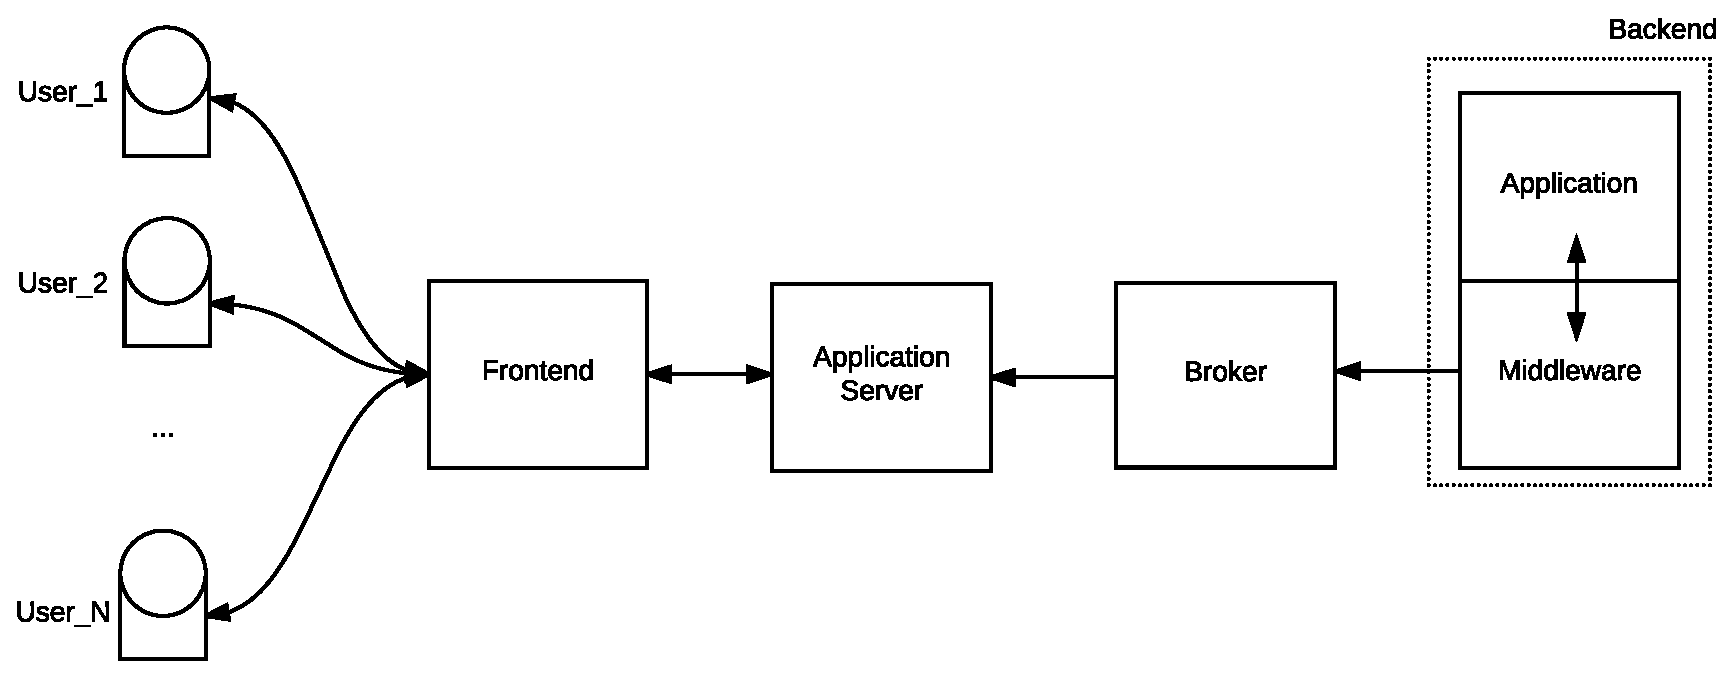
\includegraphics[scale=0.5,keepaspectratio]
    {images/solution/overall-arch.eps}
  \caption{Overall system architecture}
  \label{fig:sd-sys-arch-overall}
\end{figure}

As we can see from Figure \ref{fig:sd-sys-arch-overall}, we have:

\begin{itemize}
  \item a \textbf{Backend}, composed by the \textbf{Application} and the
    \textbf{Middleware} layers;
  \item the \textbf{Application Server}, which is responsible of handling
    information that arrives from the backend and to serve it to the frontend;
  \item a \textbf{Frontend}, which offers streaming services to end users.
\end{itemize}

Each one of these architectural macro-components can be distributed as well: we
focused our efforts on distributing the backend over multiple computation nodes
by using a \textit{2D-wrap-around topology}.
We thought this is an interesting approach to distribute our system since it
fits perfectly the way we can divide a simulated city, besides the fact this is
a topology which scales well when it comes to distribute network traffic.

In particular, we think this topology fits our needs because in our city the
most frequent application-level actions which spans over multiple nodes are
represented by a traveller which moves from a district to (obviously) an
adjacent one to continue its travel.
Therefore, if adjacent backend nodes contain adjacent districts we are able to
avoid a significant amount of unnecessary network traffic. In Figure
\ref{fig:sd-sys-arch-topology} we show a sample city, in which each district
$D_i$ is a backend node and the edges starting from each district are the links
between backend nodes:

\begin{figure}[H]
  \centering
  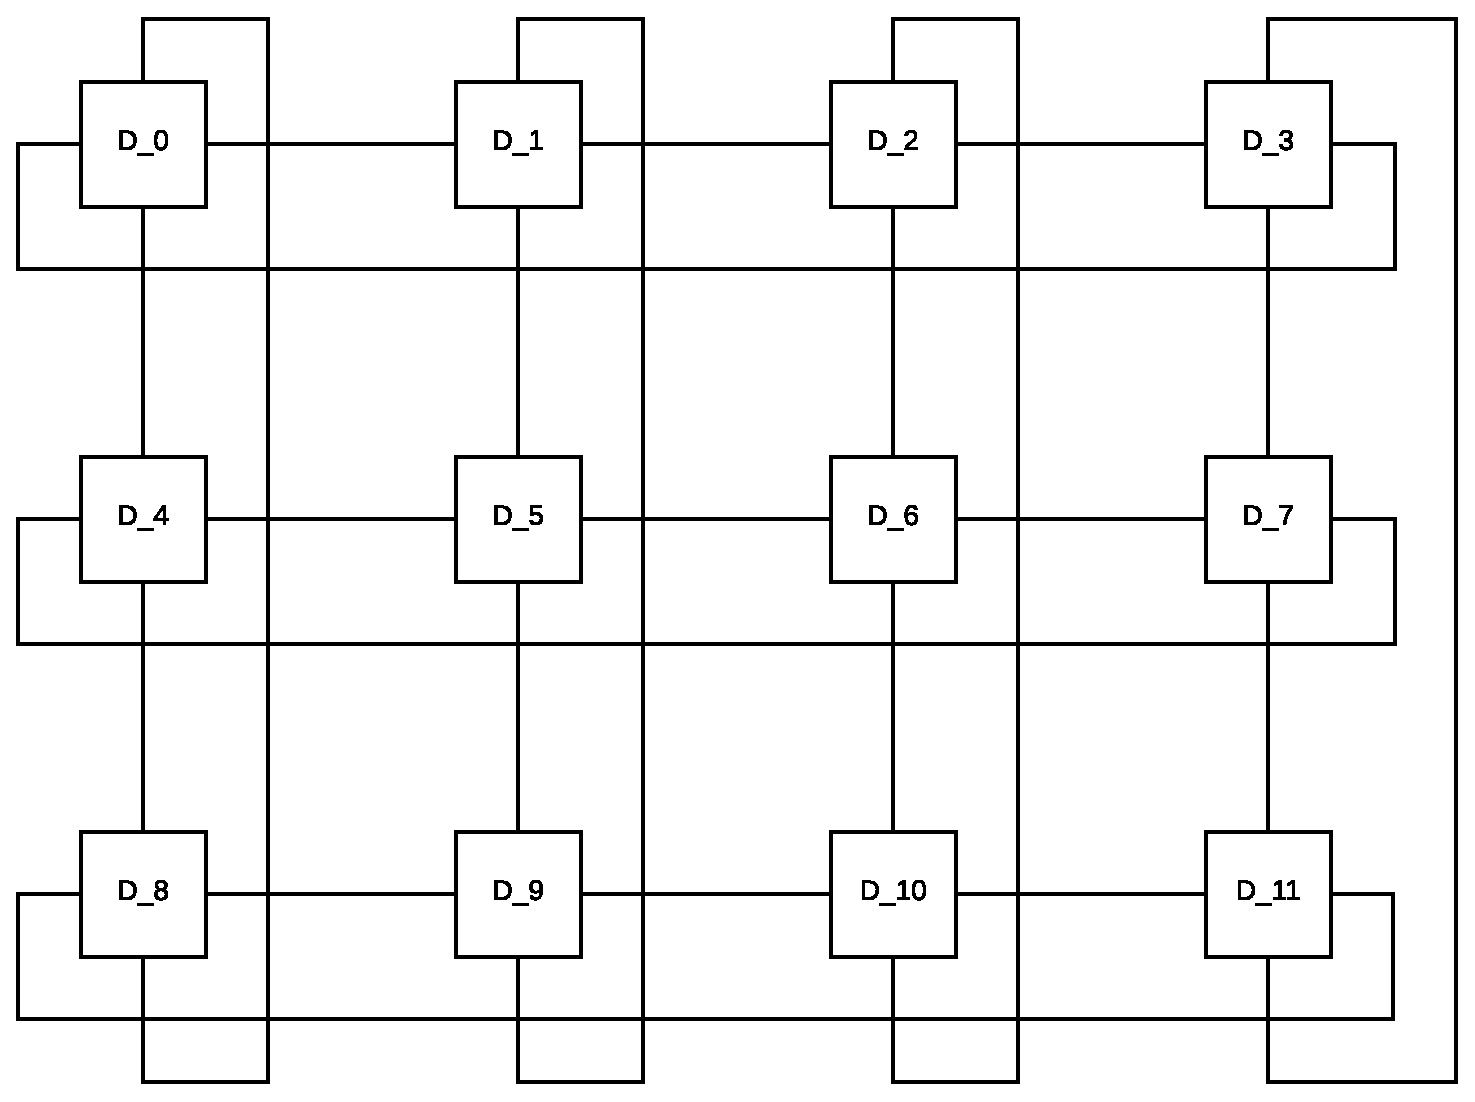
\includegraphics[scale=0.5,keepaspectratio]
    {images/solution/topology.eps}
  \caption{Sample topology for our system}
  \label{fig:sd-sys-arch-topology}
\end{figure}
